\section{Evaluation}
\label{sec:evaluation}
%
\subsection{Methodology}
\label{sec:method}

%
\niparagraph{Models and datasets.}
%
We evaluate 2.7B parameter SU-LLMs--specifically
RetNet~\cite{retnet}, GLA~\cite{gated_linear_attention},
HGRN2~\cite{hgrn2}, and Mamba-2~\cite{mamba2}--as well as
Zamba2~\cite{zamba2}, a 7B parameter hybrid transformer-Mamba-2 model.
%
For each model family, we selected the largest publicly available
pretrained architectures.
%
To provide a baseline with traditional attention-based LLM,
we also evaluate 7B parameter OPT~\cite{zhang2022opt} model.
%
To quantify the impact of state quantization on model accuracy, we
utilize standard benchmarks widely adopted in LLM evaluations:
WikiText-2~\cite{merity2016pointer}, PIQA~\cite{Bisk2020},
Lambda~\cite{paperno-EtAl:2016:P16-1},
HellaSwag~\cite{zellers2019hellaswag}, ARC-Easy~\cite{allenai:arc},
ARC-Challenge~\cite{allenai:arc}, and Winogrande~\cite{sakaguchi2021winogrande}.
%
We use perplexity and accuracy as evaluation metrics for WikiText-2
and the others, respectively.
%
Additionally, to evaluate performance at large scale, we scale the
models to 70B parameters.
%
Following established practices~\cite{scaling_laws}, we
proportionally scale both the number of layers and hidden dimensions
to reach approximately 70B parameters.
%
Based on prior findings that increasing state-update head count may
degrade perplexity~\cite{gated_linear_attention}, we retain the
original number of state-update heads and align both $dim_{head}$ and
$dim_{state}$ with the number of heads and hidden dimensions.
%

%
\niparagraph{Baselines.}
%
We evaluate \sysname{} against several baseline systems: an NVIDIA A100
GPU 80GB (\textbf{GPU}), the same GPU configuration but using
\texttt{int8} state quantization matching \sysname{}'s bitwidth
(\textbf{GPU+Q}), and the GPU system with an HBM-PIM~\cite{hbm_pim}
(\textbf{GPU+PIM}).
%
Both \sysname{} and GPU+PIM systems adopt 40 HBM2E-based PIM memory
modules operating at 1,512MHz, matching the bandwidth of the original
A100 GPU memory.
%
Given that SPU has a clock cycle of $t_{CCD\_L}$ (4 memory
bus cycles), its frequency is 378MHz, which is consistent with prior
work~\cite{hbm_pim}.
%
The HBM-PIM is designed using a time-multiplexed design that places a
\texttt{fp16} processing unit spanning two banks without the access
interleaving technique of \sysname{}.
%
This results in an area overhead comparable to that of \sysname{} PIM.
%

%
For small scale models, all evaluated systems utilize a single GPU,
as these models comfortably fit within one GPU's memory capacity.
%
For large scale models, all systems employ eight GPUs interconnected
through a high-bandwidth network analogous to the NVIDIA DGX A100 system.
%
We use NVLink3 as the interconnect for GPU-to-GPU
communication, providing a bandwidth of 600GB/s, and the models are
partitioned using tensor parallelism.
%

%
\niparagraph{Cycle-accurate simulator.}
%
We develop an in-house cycle-accurate simulator based on
Ramulator2~\cite{luo2023ramulator2} to evaluate the performance and
energy efficiency of the PIM subsystem, incorporating existing DRAM
timing constraints and refresh schemes.
%
We model other system components including GPUs and NVLink by
extending an open source simulator~\cite{park2024attacc}.
%
We refer to the activation and read energy of HBM from the previous
work~\cite{fine_grained_dram}.
%
Detailed HBM configurations are presented in Table~\ref{tab:specs}.
%

%
\niparagraph{Area and power.}
%
We synthesize \sysname{} accelerator using Synopsys Design Compiler
with the FreePDK 45nm technology node~\cite{freepdk}, scaling area
and power values to 10nm using the DeepScaleTool~\cite{9401196}.
%
The same procedure is applied to the HBM-PIM, with components sourced
from the Synopsys DesignWare libraries.
%
Scaling follows methods from prior PIM works, considering that memory
processes are 10$\times$ less dense than logic processes of the same
feature size~\cite{park2024attacc}.
%
SRAM-based buffers are modeled using CACTI7~\cite{cacti7} at 22nm,
then scaled to 10nm.
%

\begingroup
\begin{table*}[t]
  \caption{Accuracy evaluation for various small scale SU-LLMs and an
  attention-based LLM}
  \label{tab:accuracy}
  \begin{center}
    \begin{tabular}{llcccccccc}
      % Head
      \toprule[1pt]
      \multirow{2}{*}{\vspace{-1.5ex}Model} &
      \multirow{2}{*}{\vspace{-1.5ex}Method} &
      Perplexity $\downarrow$ &
      \multicolumn{7}{c}{Accuracy $\uparrow$ (\%)} \\
      \cmidrule(lr){3-3} \cmidrule(lr){4-10}
      & & WikiText-2 & Piqa & Lambada & HellaSwag & ARC-E & ARC-C &
      WinoGrande & Geomean \\

      % RetNet
      \midrule[1pt]
      \multirow{2}{*}{RetNet} & GPU & \textbf{15.83} & \textbf{72.3}
      & \textbf{44.0} & \textbf{42.0} & 59.5 & 25.5 &
      53.1 & 47.0 \\ & \sysname{} & 15.95 &
      \textbf{72.3} & 43.7 & 41.9 & \textbf{59.7} & \textbf{25.8} &
      \textbf{53.7} & \textbf{47.1}~\textcolor{black}{(+0.1)} \\

      % GLA
      \midrule
      \multirow{2}{*}{GLA} & GPU & \textbf{15.54} & \textbf{71.6} &
      \textbf{43.8} & 41.8 & \textbf{59.1} & \textbf{26.7} &
      \textbf{55.4} & \textbf{47.5} \\ &
      \sysname{} & 15.57 & 71.5 & 43.4 & \textbf{41.9} & \textbf{59.1}
      & \textbf{26.7} & 55.2 &
      47.4~\textcolor{black}{(--0.1)}\\

      % HGRN2
      \midrule
      \multirow{2}{*}{HGRN2} & GPU & \textbf{14.48} &
      \textbf{73.1} & \textbf{48.5} & 44.6 & \textbf{60.7} & \textbf{25.3} &
      54.7 & \textbf{48.6} \\
      & \sysname{} & 15.09 & 73.0 & \textbf{48.5} &
      \textbf{44.8} & 60.3 & 25.2 & \textbf{55.0} &
      \textbf{48.6}~\textcolor{black}{(+0.0)}\\

      % Mamba-2
      \midrule
      \multirow{2}{*}{Mamba-2} & GPU & \textbf{11.46} &
      \textbf{76.4} & \textbf{59.6} & \textbf{49.6} & \textbf{69.4} &
      \textbf{33.2} & \textbf{64.0} & \textbf{56.7} \\
      & \sysname{} & 11.51 & 76.3 & 59.4 & \textbf{49.6} & 69.3 &
      \textbf{33.2} & 63.9 & 56.6~\textcolor{black}{(--0.1)} \\

      % Zamba-2
      \midrule
      \multirow{2}{*}{Zamba2} & GPU & \textbf{5.94} &
      \textbf{78.9} & \textbf{64.9} & \textbf{63.8} & \textbf{78.9} &
      \textbf{53.8} & \textbf{77.7} & \textbf{69.0} \\
      & \sysname{} & 5.96 & 78.6 & 64.4 & 63.7 & 78.4
      & \textbf{53.8} & 77.1 & 68.7~\textcolor{black}{(--0.3)}\\

      % OPT
      \midrule
      \multirow{2}{*}[-2pt]{OPT} & GPU & \textbf{12.29} & \textbf{76.2} &
      \textbf{63.3} & \textbf{50.5} & \textbf{65.6} & \textbf{30.6} & 65.1 &
      \textbf{56.3} \\ & \sysname{} & \textbf{12.29} & 76.1 & 63.2 &
      \textbf{50.5} & \textbf{65.6} & 30.3 & \textbf{65.2} &
      56.2~\textcolor{black}{(--0.1)} \\

      \bottomrule[1pt]
    \end{tabular}
  \end{center}
\end{table*}
\endgroup


%
\subsection{Results}
\label{subsec:result}
\niparagraph{Throughput.}
%
Figure~\ref{fig:performance_end_to_end} reports the normalized
token-generation throughput across various SU-LLMs and an
attention-based LLM using (2,048, 2,048) input/output sequence lengths.
%
The GPU+Q system achieves an average of 1.4$\times$ higher
throughput over the GPU baseline due to halving the state size.
%
Interestingly, GPU+PIM also achieves 1.4$\times$
throughput improvement over GPU, matching or occasionally
underperforming compared to GPU+Q despite leveraging PIM.
%
This occurs because HBM-PIM employs a time-multiplexed design without
\sysname{}’s access interleaving, causing state update operations to
span multiple cycles.
%
Consequently, even with PIM, internal bandwidth is underutilized,
yielding sub-optimal performance.
%
Furthermore, GPU+PIM processes twice as much data compared to GPU+Q,
as it uses \texttt{fp16} states rather than 8-bit formats.
%
In contrast, \sysname{} consistently outperforms GPU and GPU+PIM,
providing average throughput gains of 1.9$\times$ and
1.4$\times$ (up to 4.1$\times$ and 2.1$\times$), respectively.
%
This superior performance results from efficiently leveraging
internal bandwidth through pipelining and access interleaving,
alongside the advantages of low-precision state representation.
%

\begin{figure}[t]
  \centering
  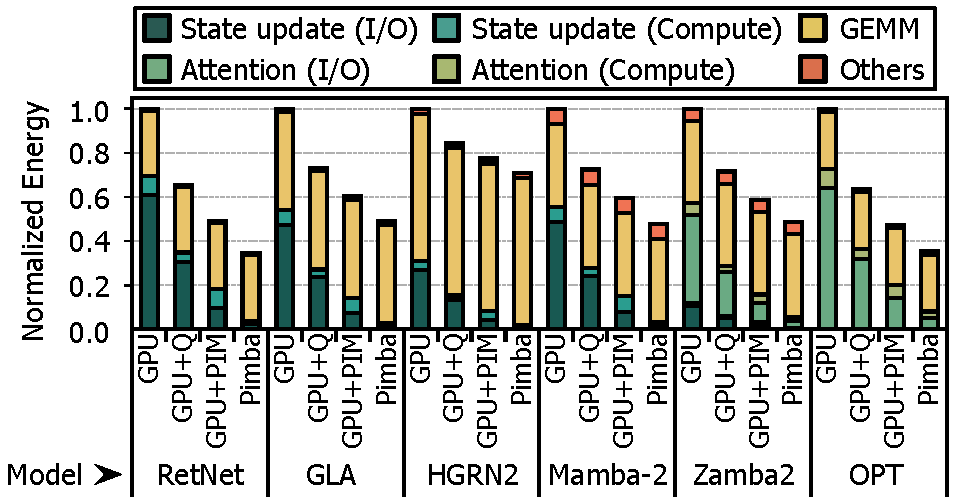
\includegraphics[width=\linewidth]{fig/eval_power.pdf}
  \caption{Normalized energy consumption of large scale SU-LLMs
    and an attention-based LLM at generation phase with
  batch size 128.}
  \label{fig:eval_power}
\end{figure}

%
\niparagraph{Latency breakdown.}
%
To identify the main contributors to throughput improvements,
Figure~\ref{fig:performance_generation} presents normalized latency
for large scale SU-LLMs and an attention-based LLM during
the generation phase.
%
As shown, \sysname{} reduces state update operation latency by
14.6$\times$ and 6.9$\times$ compared to GPU and GPU+PIM,
respectively, highlighting its efficient handling of state updates.
%
Additionally, the results show greater overall latency reduction for
larger batch sizes and models dominated by state update operations.
%
For instance, HGRN2 with a batch size of 32 spends only 14\% of its
latency on state updates, resulting in a modest 1.2$\times$ latency reduction.
%
In contrast, RetNet with a batch size of 128 allocates 74\% of its
latency to state updates, achieving a substantial 3.2$\times$ latency reduction.
%
Moreover, \sysname{} achieves latency reductions for attention
operations by 6.3$\times$ and 2.1$\times$ compared to GPU and
GPU+PIM, respectively, effectively accelerating
attention-dominated hybrid models such as Zamba2 and the
attention-based OPT.
%
Notably, the latency reduction for attention operations in \sysname{}
is smaller compared to state updates.
%
This is due to attention operations primarily consisting of GEMV
computations without requiring write operations, thus limiting the
benefits of \sysname{}’s pipelined design and access interleaving.
%
Nevertheless, by employing the \texttt{MX8} format, \sysname{} achieves
a 2.1$\times$ attention latency reduction over GPU+PIM,
demonstrating robust performance in hybrid models as well.
%

\begingroup
\begin{table}[t]
  \small
  \caption{Area and power comparison.}
  \label{tab:area}
  \begin{center}
    \begin{tabular}{ccc}
      \toprule[1pt]
      \textbf{Parameters} & \textbf{\sysname{}} & \textbf{HBM-PIM} \\

      \midrule[1pt]
      Compute area ($mm^2$) & 0.053 & 0.042 \\
      \midrule
      Buffer area ($mm^2$) & 0.039 & 0.039 \\
      \midrule
      Total area ($mm^2$) & 0.092 & 0.081 \\
      \midrule
      Area overhead (\%) & 13.4 & 11.8 \\
      \midrule
      Compute power dissipation (mW) & 8.2908 & 6.028 \\
      \bottomrule[1pt]
    \end{tabular}
  \end{center}
\end{table}
\endgroup


%
\niparagraph{Energy consumption.}
%
Figure~\ref{fig:eval_power} presents the normalized energy
consumption breakdown of large scale SU-LLMs and an
attention-based LLM with a batch size of 128 during the generation phase.
%
The results show that \sysname{} achieves an average of
2.2$\times$ lower energy consumption compared to GPU,
demonstrating its cost-effectiveness for SU-LLM serving.
%
These improvements stem from reducing the amount of state and KV
cache transfer between the GPU and memory while performing state
update operations within the PIM itself.
%
Additionally, \sysname{} exhibits an average of 1.3$\times$ lower
energy consumption compared to GPU+PIM, attributed to \sysname{}’s use
of the \texttt{MX8} which significantly reduces transfer between the
GPU as well as computation time.
%

\niparagraph{Accuracy.}
%
Table~\ref{tab:accuracy} summarizes the accuracy results comparing
\sysname{} with the GPU baseline for various small scale SU-LLMs.
%
Experimental results indicate that despite the use of \texttt{MX8}
quantization, \sysname{} achieves comparable accuracy to the GPU baseline.
%
This is because the use of \texttt{MX8}, which has a high mantissa
bit-width, combined with stochastic rounding, significantly mitigates
swamping effects during continuous state updates.
%
In conclusion, given the hardware efficiency of \texttt{MX8}, the
results affirm that \texttt{MX8} is an attractive choice to reduce
area overhead for implementing SPE, while offering a negligible
impact on the LLM accuracy.
%

%
\niparagraph{Area.}
%
To assess the practicality of \sysname{}, we measure the area and power
consumption of \sysname{} and HBM-PIM.
%
Table~\ref{tab:area} presents the results.
%
For a fair comparison, HBM-PIM is optimized for state update
computations by retaining only the essential components while
reducing or removing others, such as shrinking internal registers and
eliminating specific control logic.
%
As indicated in the table, \sysname{} adheres to PIM area constraints,
with an area overhead of 13.4\%, well below the 25\% maximum logic
ratio recommended by prior work~\cite{newton}.
%
Although \sysname{} incurs an area overhead approximately 1.5\% larger
than HBM-PIM, this increase is justified by delivering up to a
2.1$\times$ throughput improvement over HBM-PIM.
%

%
\begin{figure}[t]
  \centering
  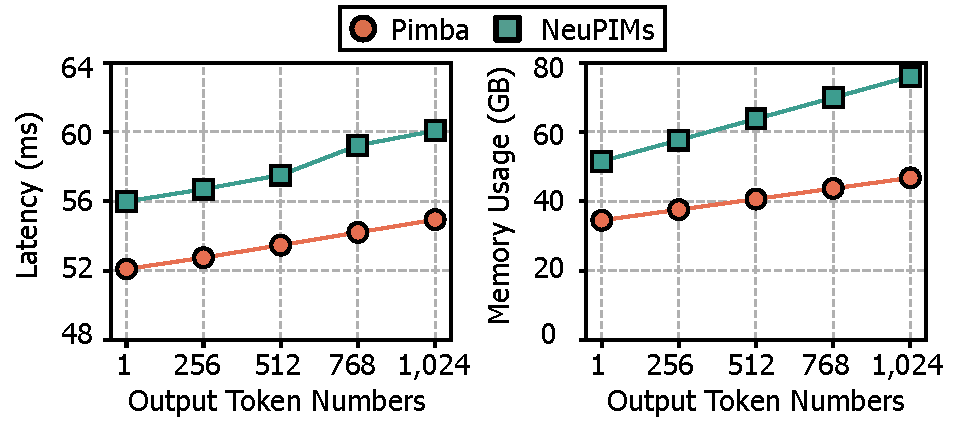
\includegraphics[width=0.9\linewidth]{fig/neupims_versus.pdf}
  \caption{Latency and memory usage of NeuPIMs and \sysname{} as the
  number of generated output tokens increases with batch size 128.}
  \label{fig:neupims_versus}
\end{figure}
%
\begin{figure}[t]
  \centering
  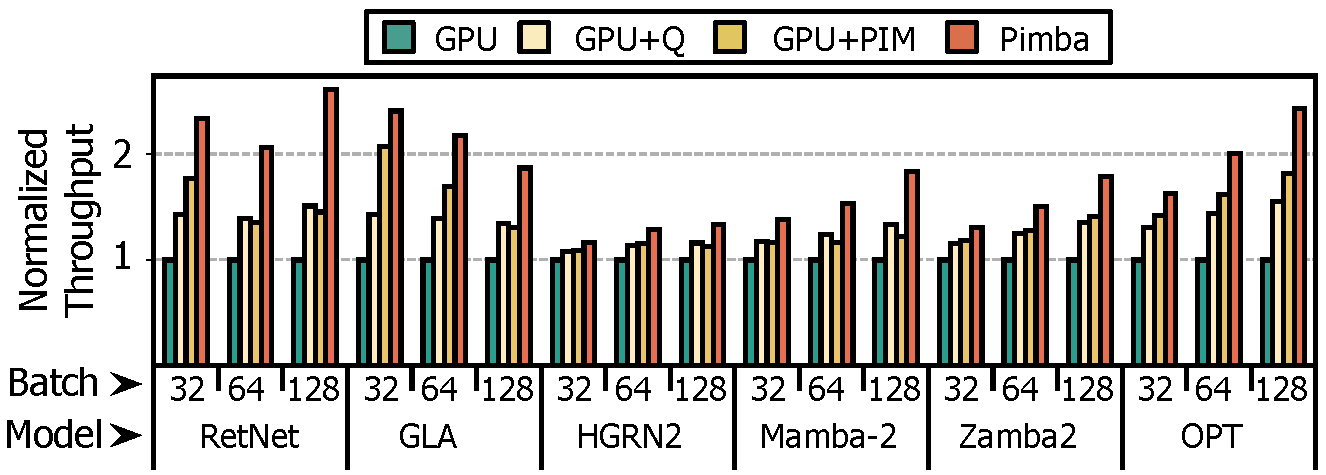
\includegraphics[width=\linewidth]{fig/performance_h100.pdf}
  \caption{Normalized generation throughput on the
  baselines and \sysname{} with NVIDIA H100 GPU settings.}
  \label{fig:performance_h100}
\end{figure}
%

%
\niparagraph{Comparison with existing PIM-enabled system.}
%
We compare the latency and memory usage of \sysname{} with
NeuPIMs~\cite{heo2024neupims}, a per-bank PIM-based acceleration
solution tailored for attention operations.
%
We use the Zamba2 70B model with batch size 128 and (1,024, 1,024)
input/output lengths.
%
Both systems use eight A100 GPUs with tensor parallelism.
%
To ensure fairness, we match the timing parameters and the number of
HBM stacks across both systems.
%
Figure~\ref{fig:neupims_versus} demonstrates that \sysname{}
consistently achieves lower latency compared to NeuPIMs.
%
This improvement arises primarily because \sysname{} efficiently
offloads state update operations onto the PIM, a critical capability
lacking in NeuPIMs.
%
Moreover, \sysname{} exhibits latency scaling similar to NeuPIMs as the
number of output tokens increases, despite utilizing half the number
of processing units, not employing dual row buffers, and foregoing
sub-batch interleaving techniques present in NeuPIMs.
%
This is enabled through optimized command scheduling and the adoption
of low precision representations for the KV cache.
%
Additionally, \sysname{} consistently maintains lower memory usage
compared to NeuPIMs, further underscoring the effectiveness of
employing low precision representations for both state data and KV cache.
%

%
\niparagraph{General adoption of \sysname{}.}
%
While our initial \sysname{} is based on the NVIDIA A100 GPU, it can
be integrated with any GPU.
%
To demonstrate this general applicability,
Figure~\ref{fig:performance_h100} presents the normalized
throughput of large scale LLMs using both baseline systems and
\sysname{} under the NVIDIA H100 GPU configuration.
%
All systems adopt 40 HBM3-based PIM modules operating at a memory
bus frequency of 2.626GHz and an SPU frequency of 657MHz, matching
the memory bandwidth of the H100.
%
They also use NVLink4 for GPU-to-GPU communication, which provides
900GB/s of bandwidth.
%
Under this setting, \sysname{} exhibits a similar acceleration trend
to that observed on the A100, consistently outperforming both the
GPU and GPU+PIM baselines by 1.8$\times$ and 1.3$\times$ on average.
%
These results demonstrate both the applicability and effectiveness
of \sysname{}, regardless of the underlying GPU platform.
